\documentclass[11pt,a4paper]{article}

\usepackage[utf8]{inputenc}
\usepackage[T1]{fontenc}
\usepackage[spanish,es-nodecimaldot]{babel}
\usepackage{lmodern}
\usepackage{geometry}
\usepackage{microtype}
\usepackage{amsmath,amssymb,bm}
\usepackage{graphicx}
\usepackage{booktabs}
\usepackage{array}
\usepackage{enumitem}
\usepackage{float}
\usepackage{caption}
\usepackage{xcolor}
\usepackage{tikz}
\usetikzlibrary{arrows.meta,positioning,calc,angles,quotes,shapes.geometric}
\usepackage[hidelinks]{hyperref}

\geometry{top=2.3cm,bottom=2.3cm,left=2.5cm,right=2.5cm}
\setlength{\parindent}{0pt}
\setlength{\parskip}{0.65em}
\setlist[itemize]{nosep,leftmargin=1.5em}
\setlist[enumerate]{nosep,leftmargin=1.7em}

\definecolor{azul}{RGB}{25,88,140}
\definecolor{naranja}{RGB}{210,105,30}
\definecolor{gris}{RGB}{245,247,249}

\newcommand{\vect}[1]{\bm{#1}}
\newcommand{\R}{\mathbb{R}}

\title{\textbf{Control LQI y cinemática inversa de un robot SCARA planar de dos grados de libertad}}
\author{Jhon}
\date{\today}

\begin{document}

\maketitle

\begin{abstract}
Se presenta el diseño y la implementación de un robot SCARA planar de dos articulaciones rotacionales. Cada articulación utiliza un motor de corriente continua con encoder, un puente H TB6612 y un controlador LQI discreto ejecutado en un Seeed Studio XIAO ESP32-S3. La computadora envía una posición cartesiana $(p_x,p_y)$ por USB; el microcontrolador verifica su validez, calcula la cinemática inversa y genera las referencias articulares. El trabajo se concentra en el modelo geométrico del brazo, las soluciones de cinemática inversa, los límites articulares y la arquitectura de software usada para controlar ambos motores en tiempo real.
\end{abstract}

\section{Introducción}

Un robot SCARA posiciona su efector mediante articulaciones que se desplazan principalmente en un plano horizontal. El prototipo desarrollado implementa el subsistema planar de dos grados de libertad, formado por dos articulaciones rotacionales. No se incluye el eje prismático vertical que aparece en un SCARA industrial completo.

El usuario especifica una coordenada cartesiana desde MATLAB. El ESP32 convierte esa coordenada en dos ángulos, controla cada motor de forma independiente y devuelve telemetría para comparar las referencias con las posiciones medidas. La posición inicial se define con los dos eslabones extendidos sobre el eje $x$.

\section{Objetivos}

\subsection{Objetivo general}

Diseñar e implementar el control de posición de un robot SCARA planar 2R, capaz de recibir una referencia cartesiana, resolver su cinemática inversa y mover ambas articulaciones dentro de límites seguros.

\subsection{Objetivos específicos}

\begin{itemize}
    \item Modelar la posición del efector final en función de $\theta_1$ y $\theta_2$.
    \item Obtener las expresiones cerradas de la cinemática inversa.
    \item Controlar cada motor mediante un LQI discreto con realimentación de encoder.
    \item Restringir ambas articulaciones al intervalo $[-\pi/2,\pi/2]$.
    \item Comunicar MATLAB y el ESP32 mediante USB Serial/JTAG.
    \item Mostrar en tiempo real las referencias, los ángulos medidos y la configuración estimada del brazo.
\end{itemize}

\section{Materiales y parámetros físicos}

\begin{table}[H]
\centering
\caption{Elementos principales del sistema.}
\begin{tabular}{>{\raggedright\arraybackslash}p{4.2cm} p{9.2cm}}
\toprule
\textbf{Elemento} & \textbf{Función} \\
\midrule
XIAO ESP32-S3 & Ejecuta las tareas FreeRTOS, la cinemática inversa, los dos controladores LQI y la comunicación USB. \\
TB6612 & Puente H doble. Gobierna el sentido de giro y el PWM de los dos motores. \\
Dos motores DC con encoder & Actúan sobre las articulaciones. El conteo efectivo usado por el programa es de $8341$ cuentas por revolución del eje de salida. \\
Brazo de dos eslabones & Primer eslabón $a_1=8.3\,\mathrm{cm}$ y segundo eslabón $a_2=10.1\,\mathrm{cm}$. \\
Fuente de potencia & Alimentación de los motores y del puente H; la lógica se conecta al nivel de $3.3\,\mathrm{V}$ del ESP32. \\
Computadora con MATLAB & Envía $(p_x,p_y)$ y presenta la telemetría en gráficas. \\
\bottomrule
\end{tabular}
\end{table}

El valor $8341$ se usa como resolución efectiva después de la reducción mecánica y de la decodificación en cuadratura. En sentido estricto, el firmware trabaja con cuentas por revolución (CPR). En el contexto del proyecto también se denomina PPR efectivo. La resolución angular es

\begin{equation}
\Delta\theta=\frac{2\pi}{8341}
=7.533\times10^{-4}\ \mathrm{rad}
\approx 0.0432^{\circ}.
\end{equation}

\section{Control de posición de cada motor}

\subsection{Modelo discreto}

La identificación del motor aproxima la dinámica de velocidad mediante

\begin{equation}
\omega[k+1]=a\,\omega[k]+b\,u[k],
\end{equation}

donde $u[k]$ es la acción normalizada aplicada al puente H. Para el modelo utilizado,

\begin{equation}
a=0.7068, \qquad b=3.0825.
\end{equation}

La posición se obtiene integrando la velocidad con un periodo de muestreo $T_s=20\,\mathrm{ms}$:

\begin{equation}
\theta[k+1]=\theta[k]+T_s\omega[k].
\end{equation}

Con $\vect{x}[k]=[\theta[k]\;\omega[k]]^T$, el modelo queda

\begin{align}
\vect{x}[k+1]&=G\vect{x}[k]+H u[k],\\
y[k]&=C\vect{x}[k],
\end{align}

con

\begin{equation}
G=
\begin{bmatrix}
1&T_s\\
0&a
\end{bmatrix},\qquad
H=
\begin{bmatrix}
0\\b
\end{bmatrix},\qquad
C=\begin{bmatrix}1&0\end{bmatrix}.
\end{equation}

\subsection{Acción integral y ley LQI}

Para eliminar error estacionario se incorpora el estado integral

\begin{equation}
v[k+1]=v[k]+e[k+1],\qquad e[k]=r[k]-y[k].
\end{equation}

El estado aumentado $\vect{\xi}[k]=[\vect{x}^T[k]\;v[k]]^T$ satisface

\begin{equation}
\vect{\xi}[k+1]=
\underbrace{\begin{bmatrix}
G&0\\-CG&1
\end{bmatrix}}_{\widehat G}
\vect{\xi}[k]
+
\underbrace{\begin{bmatrix}
H\\-CH
\end{bmatrix}}_{\widehat H}u[k]
+
\underbrace{\begin{bmatrix}0\\0\\1\end{bmatrix}}_{H_r}r[k+1].
\end{equation}

La ley implementada es

\begin{equation}
u[k]=-K_{\theta}\theta[k]-K_{\omega}\omega[k]+K_i v[k],
\end{equation}

con

\begin{equation}
K_{\theta}=8.5621,\qquad
K_{\omega}=0.3637,\qquad
K_i=1.9635.
\end{equation}

Estas ganancias se aplican por separado a los dos motores. El LQI se complementa con saturación $u\in[-0.15,0.15]$, anti-windup, filtro de velocidad y una rampa que evita cambios bruscos. La figura~\ref{fig:calculos-lqi} reúne el planteamiento usado para obtener el controlador.

\begin{figure}[H]
\centering
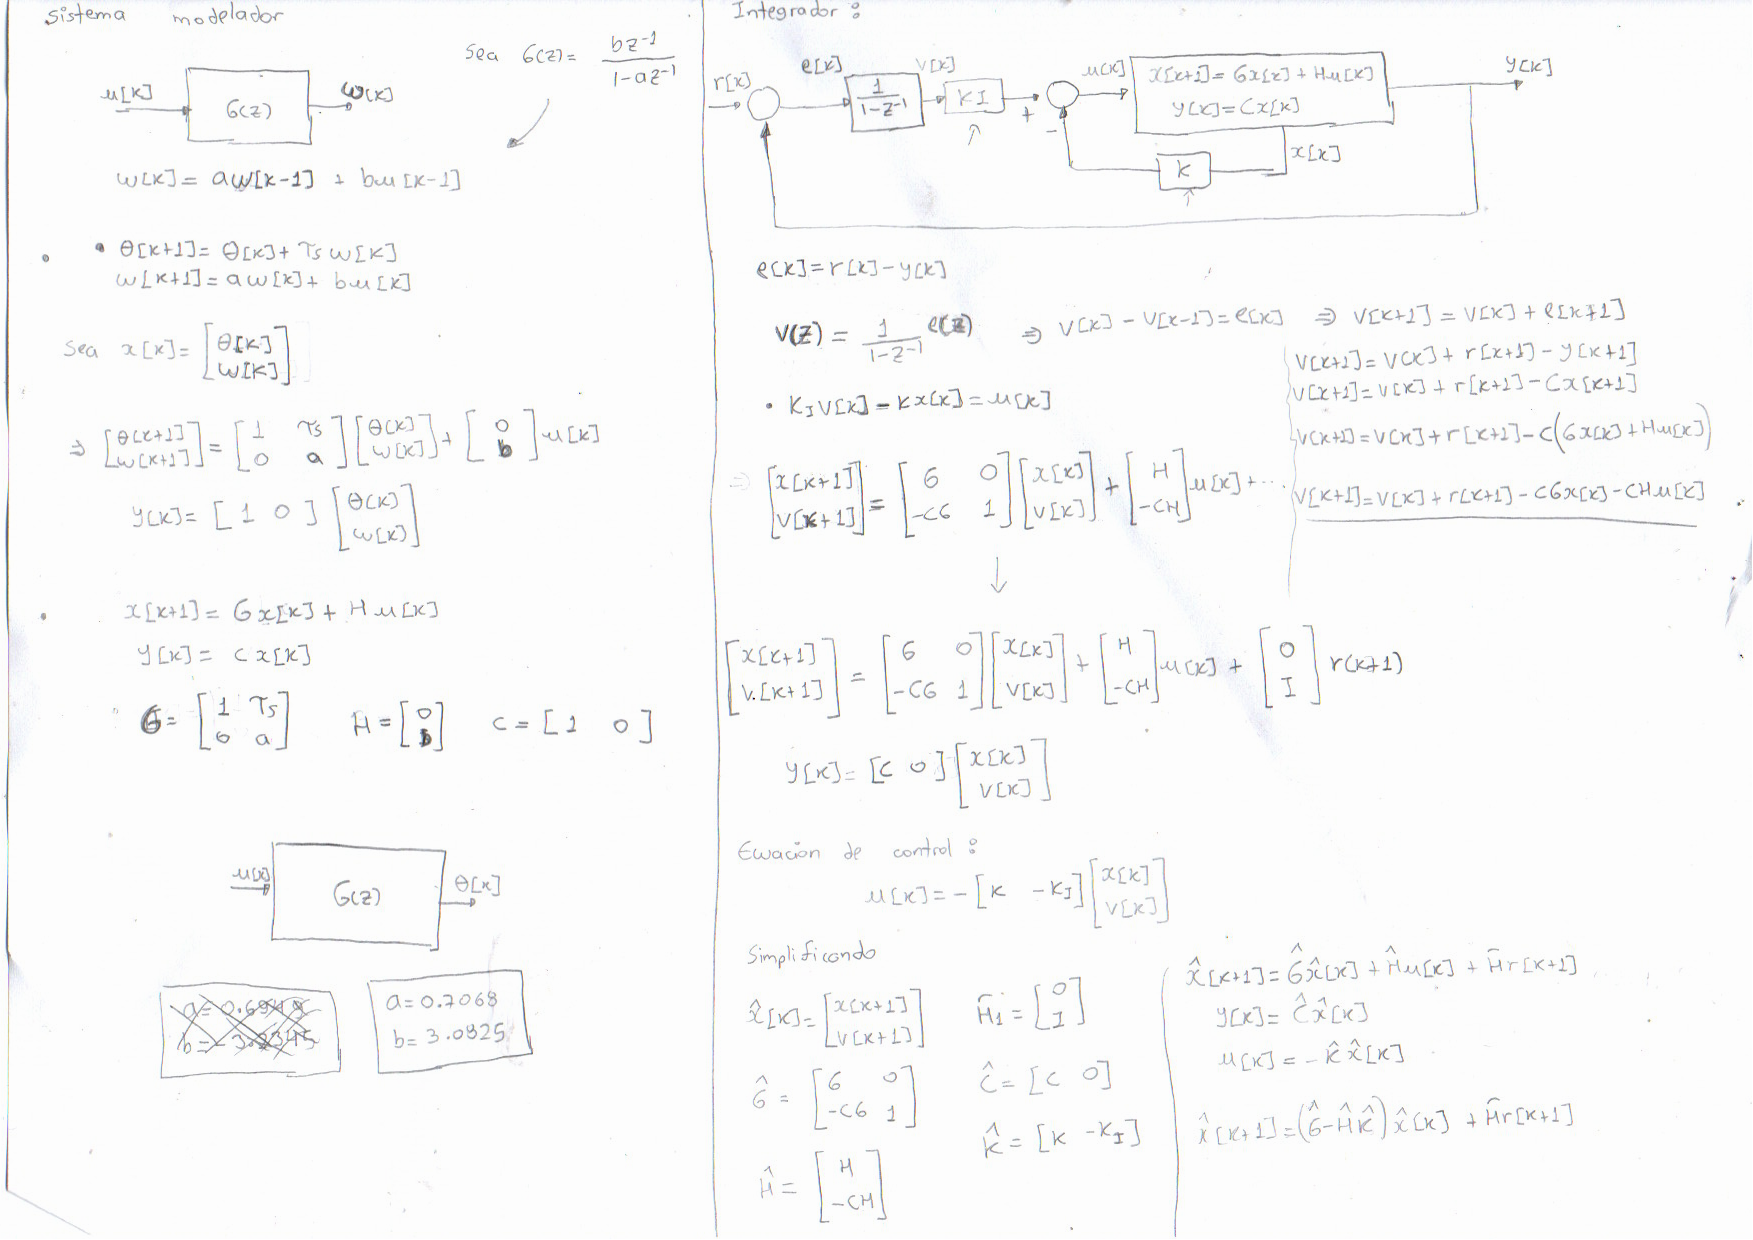
\includegraphics[width=\textwidth]{figuras/calculos_lqi.png}
\caption{Desarrollo del modelo discreto y del estado integral del controlador LQI.}
\label{fig:calculos-lqi}
\end{figure}

\begin{table}[H]
\centering
\caption{Parámetros implementados en cada controlador.}
\begin{tabular}{lc}
\toprule
\textbf{Parámetro} & \textbf{Valor} \\
\midrule
Periodo de muestreo & $20\,\mathrm{ms}$ \\
PWM & $60\,\mathrm{kHz}$, resolución de 10 bits \\
Control normalizado & $-0.15\leq u\leq 0.15$ \\
Variación máxima por muestra & $0.04$ \\
Pausa antes de invertir el giro & 5 muestras ($100\,\mathrm{ms}$) \\
Filtro de velocidad & $\omega_f[k]=0.60\omega_f[k-1]+0.40\omega_m[k]$ \\
Tolerancia de entrada en posición & $0.035\,\mathrm{rad}$ \\
Tolerancia de salida en posición & $0.040\,\mathrm{rad}$ \\
Tiempo de confirmación & 5 muestras ($100\,\mathrm{ms}$) \\
\bottomrule
\end{tabular}
\end{table}

La posición y la velocidad se calculan directamente desde el encoder:

\begin{align}
\theta[k]&=\frac{2\pi}{N}\,n[k],\\
\omega_m[k]&=\frac{2\pi}{N T_s}\left(n[k]-n[k-1]\right),
\end{align}

donde $N=8341$ y $n[k]$ es el conteo acumulado.

\section{Modelo geométrico del robot SCARA 2R}

\subsection{Definición de coordenadas}

El brazo tiene dos articulaciones rotacionales. El motor B mueve la primera articulación y representa $\theta_1$; el motor A mueve la segunda y representa $\theta_2$. Los ángulos positivos se miden en sentido antihorario, por lo que una referencia $p_y>0$ corresponde a un movimiento hacia arriba en el plano cartesiano.

La figura~\ref{fig:brazo-2r} muestra la geometría adoptada.

\begin{figure}[H]
\centering
\includegraphics[width=0.82\textwidth]{figuras/SCARA.jpeg}
\caption{Modelo planar de dos eslabones utilizado en la implementación.}
\label{fig:brazo-2r}
\end{figure}

La configuración inicial es

\begin{equation}
\theta_1=0,\qquad \theta_2=0.
\end{equation}

En consecuencia, el brazo comienza extendido:

\begin{equation}
p_x=a_1+a_2=18.4\,\mathrm{cm},\qquad p_y=0.
\end{equation}

Los encoders son incrementales. Por ello, el operador debe colocar físicamente el brazo en esa configuración antes de encender o reiniciar el sistema. El firmware pone ambos contadores en cero durante la inicialización, pero no puede determinar una posición absoluta sin sensores de referencia.

\subsection{Parámetros de Denavit--Hartenberg}

Para el mecanismo planar se usan los parámetros de la tabla~\ref{tab:dh}. Los desplazamientos $d_i$ y los giros $\alpha_i$ son cero.

\begin{table}[H]
\centering
\caption{Parámetros DH del brazo 2R.}
\label{tab:dh}
\begin{tabular}{ccccc}
\toprule
$i$ & $a_i$ & $\alpha_i$ & $d_i$ & $\theta_i$ \\
\midrule
1 & $8.3\,\mathrm{cm}$ & $0$ & $0$ & $\theta_1$ \\
2 & $10.1\,\mathrm{cm}$ & $0$ & $0$ & $\theta_2$ \\
\bottomrule
\end{tabular}
\end{table}

La transformación de cada eslabón es

\begin{equation}
{}^{i-1}T_i=
\begin{bmatrix}
\cos\theta_i&-\sin\theta_i&0&a_i\cos\theta_i\\
\sin\theta_i& \cos\theta_i&0&a_i\sin\theta_i\\
0&0&1&0\\
0&0&0&1
\end{bmatrix}.
\end{equation}

El producto ${}^{0}T_2={}^{0}T_1{}^{1}T_2$ resulta

\begin{equation}
{}^{0}T_2=
\begin{bmatrix}
c_{12}&-s_{12}&0&a_1c_1+a_2c_{12}\\
s_{12}& c_{12}&0&a_1s_1+a_2s_{12}\\
0&0&1&0\\
0&0&0&1
\end{bmatrix},
\end{equation}

donde $c_1=\cos\theta_1$, $s_1=\sin\theta_1$, $c_{12}=\cos(\theta_1+\theta_2)$ y $s_{12}=\sin(\theta_1+\theta_2)$.

\subsection{Cinemática directa}

La posición del efector final se obtiene de la última columna de ${}^{0}T_2$:

\begin{align}
p_x&=a_1\cos\theta_1+a_2\cos(\theta_1+\theta_2),\label{eq:px}\\
p_y&=a_1\sin\theta_1+a_2\sin(\theta_1+\theta_2).\label{eq:py}
\end{align}

La orientación del segundo eslabón respecto al eje $x$ es

\begin{equation}
\phi=\theta_1+\theta_2.
\end{equation}

Estas ecuaciones se usan en MATLAB para reconstruir la postura medida a partir de la telemetría.

\subsection{Cinemática inversa}

La cinemática inversa determina $(\theta_1,\theta_2)$ a partir de $(p_x,p_y)$. Al elevar al cuadrado y sumar las ecuaciones~\eqref{eq:px} y~\eqref{eq:py}, se obtiene

\begin{equation}
p_x^2+p_y^2=a_1^2+a_2^2+2a_1a_2\cos\theta_2.
\end{equation}

Por tanto,

\begin{equation}
D=\cos\theta_2=
\frac{p_x^2+p_y^2-a_1^2-a_2^2}{2a_1a_2}.
\label{eq:D}
\end{equation}

Existe una solución geométrica real solo si

\begin{equation}
-1\leq D\leq 1.
\end{equation}

Las dos configuraciones posibles se expresan como

\begin{equation}
\theta_2=\operatorname{atan2}\left(s\sqrt{1-D^2},D\right),
\label{eq:theta2}
\end{equation}

donde $s=+1$ selecciona una rama y $s=-1$ la configuración reflejada. Una vez calculado $\theta_2$,

\begin{equation}
\theta_1=\operatorname{atan2}(p_y,p_x)-
\operatorname{atan2}\left(a_2\sin\theta_2,
a_1+a_2\cos\theta_2\right).
\label{eq:theta1}
\end{equation}

El programa selecciona

\begin{equation}
s=\begin{cases}
+1,&p_y\geq 0,\\
-1,&p_y<0.
\end{cases}
\end{equation}

Así, los objetivos $(p_x,+p_y)$ y $(p_x,-p_y)$ generan posturas aproximadamente simétricas respecto al eje $x$. Un valor positivo de $p_y$ mueve el brazo hacia arriba y uno negativo lo mueve hacia abajo.

\subsection{Límites articulares y espacio de trabajo}

Cada articulación está limitada por software:

\begin{equation}
-\frac{\pi}{2}\leq\theta_1\leq\frac{\pi}{2},
\qquad
-\frac{\pi}{2}\leq\theta_2\leq\frac{\pi}{2}.
\label{eq:limits}
\end{equation}

Sin límites articulares, el alcance radial de un brazo 2R es

\begin{equation}
|a_2-a_1|\leq \rho \leq a_1+a_2,
\qquad \rho=\sqrt{p_x^2+p_y^2},
\end{equation}

lo que produciría

\begin{equation}
1.8\,\mathrm{cm}\leq\rho\leq18.4\,\mathrm{cm}.
\end{equation}

Sin embargo, el límite $|\theta_2|\leq\pi/2$ implica $\cos\theta_2\geq0$. Al sustituirlo en la ecuación radial,

\begin{equation}
\rho_{\min}=\sqrt{a_1^2+a_2^2}
=\sqrt{8.3^2+10.1^2}
\approx13.07\,\mathrm{cm}.
\end{equation}

Por tanto, una condición radial necesaria en el programa es

\begin{equation}
13.07\,\mathrm{cm}\leq\rho\leq18.4\,\mathrm{cm}.
\end{equation}

Esta condición no es suficiente: la solución también debe respetar el límite de $\theta_1$. El firmware calcula los ángulos y rechaza cualquier punto que viole la ecuación~\eqref{eq:limits}. Además, durante el movimiento anula el PWM que intente aumentar un ángulo situado en su límite.

\subsection{Jacobiano y configuraciones singulares}

Al derivar las ecuaciones de posición se obtiene

\begin{equation}
\begin{bmatrix}
\dot p_x\\\dot p_y
\end{bmatrix}
=J(\vect{q})
\begin{bmatrix}
\dot\theta_1\\\dot\theta_2
\end{bmatrix},
\end{equation}

con

\begin{equation}
J(\vect{q})=
\begin{bmatrix}
-a_1\sin\theta_1-a_2\sin(\theta_1+\theta_2)&-a_2\sin(\theta_1+\theta_2)\\
a_1\cos\theta_1+a_2\cos(\theta_1+\theta_2)& a_2\cos(\theta_1+\theta_2)
\end{bmatrix}.
\end{equation}

Su determinante es

\begin{equation}
\det J=a_1a_2\sin\theta_2.
\end{equation}

El brazo está en una singularidad cuando $\theta_2=0$, es decir, cuando los eslabones están alineados. La posición inicial extendida es singular en velocidad cartesiana: pequeños cambios cartesianos cerca de $\rho=18.4\,\mathrm{cm}$ pueden exigir cambios articulares relativamente grandes. La implementación utiliza las expresiones cerradas~\eqref{eq:theta2} y~\eqref{eq:theta1}, por lo que no invierte el Jacobiano, pero aun así conviene evitar referencias exactamente sobre el borde del alcance durante las pruebas dinámicas.

\subsection{Correspondencia entre el modelo y los motores}

La asignación física es

\begin{equation}
\theta_1\longleftrightarrow\text{motor B},\qquad
\theta_2\longleftrightarrow\text{motor A}.
\end{equation}

En el montaje, el conteo positivo de ambos encoders corresponde al sentido negativo del modelo geométrico. La conversión usada es

\begin{equation}
\theta_{1,\mathrm{modelo}}=-\theta_{B,\mathrm{encoder}},
\qquad
\theta_{2,\mathrm{modelo}}=-\theta_{A,\mathrm{encoder}}.
\end{equation}

Esta transformación permite conservar la convención habitual: giro antihorario positivo y $p_y>0$ hacia arriba, sin modificar el conteo interno ni la ley de control.

\section{Arquitectura del software}

El firmware se divide en componentes y tareas. Los componentes \texttt{pwm\_ctrl}, \texttt{lqi} y \texttt{robotica} encapsulan el hardware, el control y la geometría, respectivamente. La aplicación \texttt{main\_lqi2.c} conecta esos módulos mediante colas de FreeRTOS.

\begin{figure}[H]
\centering
\resizebox{\textwidth}{!}{%
\begin{tikzpicture}[
    node distance=7mm and 9mm,
    block/.style={draw,rounded corners,fill=gris,align=center,minimum height=9mm,text width=28mm},
    queue/.style={draw,fill=blue!7,align=center,minimum height=8mm,text width=25mm},
    hw/.style={draw,fill=orange!10,align=center,minimum height=9mm,text width=27mm},
    line/.style={-{Latex[length=2mm]},thick}
]
    \node[block] (matlab) {MATLAB\\$(p_x,p_y)$};
    \node[block,right=of matlab] (usb) {\texttt{vTaskUSB}\\valida CRLF};
    \node[queue,right=of usb] (qxy) {cola USB\\último objetivo};
    \node[block,right=of qxy] (ik) {\texttt{vTaskReference}\\cinemática inversa};

    \node[queue,below right=10mm and -2mm of ik] (q1) {cola $r_1$\\$\theta_2$};
    \node[queue,above right=10mm and -2mm of ik] (q2) {cola $r_2$\\$\theta_1$};
    \node[block,right=of q2] (lqiB) {LQI motor B\\articulación 1};
    \node[block,right=of q1] (lqiA) {LQI motor A\\articulación 2};
    \node[hw,right=of lqiB] (tbB) {TB6612\\canal B};
    \node[hw,right=of lqiA] (tbA) {TB6612\\canal A};

    \node[hw,right=of tbB] (mB) {Motor B\\encoder};
    \node[hw,right=of tbA] (mA) {Motor A\\encoder};

    \node[queue,below=15mm of q1] (qt) {cola de\\telemetría};
    \node[block,left=of qt] (tx) {\texttt{vTaskUart}\\formato ARM};

    \draw[line] (matlab)--(usb);
    \draw[line] (usb)--(qxy);
    \draw[line] (qxy)--(ik);
    \draw[line] (ik)--(q2);
    \draw[line] (ik)--(q1);
    \draw[line] (q2)--(lqiB);
    \draw[line] (q1)--(lqiA);
    \draw[line] (lqiB)--node[above]{PWM}(tbB);
    \draw[line] (lqiA)--node[above]{PWM}(tbA);
    \draw[line] (tbB)--(mB);
    \draw[line] (tbA)--(mA);
    \draw[line] (mB.north) |- node[pos=0.22,right]{PCNT} (lqiB.north);
    \draw[line] (mA.south) |- node[pos=0.22,right]{PCNT} (lqiA.south);
    \draw[line] (lqiA.south) |- (qt.east);
    \draw[line] (lqiB.south) |- (qt.east);
    \draw[line] (qt)--(tx);
    \draw[line] (tx.west) -| node[pos=0.25,below]{USB} (matlab.south);
\end{tikzpicture}
}%
\caption{Flujo de referencias, control y telemetría.}
\label{fig:arquitectura}
\end{figure}

\begin{table}[H]
\centering
\caption{Responsabilidad de las tareas principales.}
\begin{tabular}{p{3.2cm}p{9.9cm}}
\toprule
\textbf{Tarea} & \textbf{Responsabilidad} \\
\midrule
\texttt{vTaskUSB} & Lee líneas \texttt{px,py\textbackslash r\textbackslash n}, valida dos números finitos y conserva el objetivo más reciente. \\
\texttt{vTaskReference} & Calcula la cinemática inversa, selecciona la rama según el signo de $p_y$, verifica $\pm\pi/2$ y entrega las referencias articulares. \\
\texttt{vTask\_Lqi1} & Controla el motor A, asociado con $\theta_2$. \\
\texttt{VTask\_Lqi2} & Controla el motor B, asociado con $\theta_1$. \\
\texttt{vTaskUart} & Combina la telemetría de ambos motores y la transmite por la consola USB. El nombre se conserva por compatibilidad, aunque la salida activa es USB Serial/JTAG. \\
\texttt{vTaskReset} & Atiende el semáforo generado por el pulsador y ordena el retorno de ambas referencias a cero. \\
\bottomrule
\end{tabular}
\end{table}

Las tareas LQI tienen prioridad 5; la cinemática inversa, prioridad 4; la comunicación y el reinicio, prioridad 3. Esta asignación favorece la periodicidad del control. Cada lazo se ejecuta cada $20\,\mathrm{ms}$ y la telemetría se reduce a una muestra cada cinco ciclos, aproximadamente $10\,\mathrm{Hz}$.

\section{Comunicación y visualización}

MATLAB transmite una referencia mediante

\begin{center}
\texttt{px,py\textbackslash r\textbackslash n}
\end{center}

y el ESP32 responde con

\begin{center}
\texttt{ARM,px,py,theta1\_ref,theta2\_ref,theta1,theta2}.
\end{center}

Las coordenadas están en centímetros y los ángulos en radianes. El script convierte los ángulos a grados para la gráfica y aplica la cinemática directa para dibujar el brazo medido junto al punto objetivo.

Como ejemplo, para $(p_x,p_y)=(13,13)\,\mathrm{cm}$ se registró

\begin{align}
\theta_{1,r}&=0.740518\,\mathrm{rad}, & \theta_1&=0.739730\,\mathrm{rad},\\
\theta_{2,r}&=0.081757\,\mathrm{rad}, & \theta_2&=0.084368\,\mathrm{rad}.
\end{align}

Los errores instantáneos correspondientes son aproximadamente

\begin{equation}
e_1=7.88\times10^{-4}\,\mathrm{rad},\qquad
e_2=-2.61\times10^{-3}\,\mathrm{rad}.
\end{equation}

\section{Implementación física}

La figura~\ref{fig:brazo-fisico} queda reservada para la fotografía final del prototipo. Para incorporarla basta guardar el archivo como \texttt{figuras/brazo\_implementado.jpg} o \texttt{figuras/brazo\_implementado.png}; no es necesario modificar el documento.

\begin{figure}[H]
\centering
\IfFileExists{figuras/brazo_implementado.jpg}{%
    \includegraphics[width=0.78\textwidth]{figuras/brazo_implementado.jpg}%
}{%
    \IfFileExists{figuras/brazo_implementado.png}{%
        \includegraphics[width=0.78\textwidth]{figuras/brazo_implementado.png}%
    }{%
        \fbox{\parbox[c][5.2cm][c]{0.78\textwidth}{\centering
        Fotografía pendiente\\[0.5em]
        Guardar como \texttt{figuras/brazo\_implementado.jpg}}}%
    }%
}
\caption{Implementación física del robot SCARA planar 2R.}
\label{fig:brazo-fisico}
\end{figure}

\section{Procedimiento de operación}

\begin{enumerate}
    \item Colocar físicamente los dos eslabones extendidos sobre el eje $x$.
    \item Encender o reiniciar el ESP32 para establecer $\theta_1=\theta_2=0$.
    \item Cerrar cualquier monitor serial que esté usando el puerto COM3.
    \item Ejecutar \texttt{usb\_esp32\_console.m} en MATLAB.
    \item Enviar un objetivo en centímetros, por ejemplo \texttt{17.0,1.5}.
    \item Verificar las referencias y los ángulos medidos antes de ordenar desplazamientos mayores.
\end{enumerate}

Se recomienda evitar cambios directos entre extremos superiores e inferiores y no usar puntos cercanos al borde de $18.4\,\mathrm{cm}$ durante las primeras pruebas.

\section{Conclusiones}

El sistema integra la geometría de un brazo 2R con dos lazos independientes de posición. La cinemática inversa convierte directamente una referencia cartesiana en referencias articulares y selecciona configuraciones simétricas para movimientos por encima y por debajo del eje $x$. Los límites de $\pm\pi/2$ reducen el espacio alcanzable, pero evitan que las articulaciones sobrepasen el intervalo mecánico definido.

La separación entre adquisición USB, cálculo de referencias, control de motores y telemetría simplifica la verificación del sistema. El uso de colas desacopla las tareas y permite que los lazos LQI mantengan su periodo de muestreo. Finalmente, la conversión de signo entre encoder y modelo conserva una representación cartesiana coherente: $p_y>0$ corresponde al movimiento físico hacia arriba.

\begin{thebibliography}{9}

\bibitem{spong}
M. W. Spong, S. Hutchinson y M. Vidyasagar,
\textit{Robot Modeling and Control}.
Wiley, 2006.

\bibitem{craig}
J. J. Craig,
\textit{Introduction to Robotics: Mechanics and Control}, 3.ª ed.
Pearson, 2005.

\bibitem{ogata}
K. Ogata,
\textit{Discrete-Time Control Systems}, 2.ª ed.
Prentice Hall, 1995.

\bibitem{tb6612}
Toshiba Electronic Devices \& Storage Corporation,
\textit{TB6612FNG: Dual DC Motor Driver IC}, hoja de datos.

\bibitem{espidf}
Espressif Systems,
\textit{ESP-IDF Programming Guide: FreeRTOS, LEDC, PCNT y USB Serial/JTAG}.

\end{thebibliography}

\end{document}
